%
% intensitaet.tex -- Paper zum Thema Optische Fourier-Transformation <opt>
%
% (c) 2023 Marco Niederberger, Yanick Schoch; OST Ostschweizer Fachhochschule
%
% !TEX root = ../../buch.tex
% !TEX encoding = UTF-8
%
\section{Intensität\label{opt:sec:intensity}}
\rhead{Intensität}

Die in \eqref{opt:equation:integral_fraunhofer} hergeleitete elektrische Feldstärke kann nicht direkt beobachtet werden.
Ein Beobachter, sei es das menschliche Auge oder ein Kamerachip, kann lediglich die Intensität einer Lichtquelle wahrnehmen.
Die Intensität im Allgemeinen ist ein Mass für die Energie pro Fläche.

In diesem Abschnitt wird ein möglicher Weg gezeigt, den Zusammenhang zwischen der elektrischen Feldstärke $E$ und der Intensität $I$ zu finden.
Diese Herangehensweise gliedert sich in zwei Abschnitte.
Zuerst wird im Abschnitt \ref{opt:subsection:poynting_vector} mittels des Poynting-Vektors der Zusammenhang zwischen $E$ und $I$ hergeleitet.
Allerdings wird dieser Ausdruck für die Intensität $I$ noch zusätzlich von der magnetischen Feldstärke $H$ abhängig sein.
Aufgrund dessen wird im darauf folgenden Abschnitt \ref{opt:subsection:wave_impedance} mit Hilfe der Wellenimpedanz gezeigt, wie diese Abhängigkeit zu beseitigen ist.

Abgeschlossen wir dieser Abschnitt mit einem Rechenbeispiel zur Beugung am Einzelspalt.

%%%%%%%%%%%%%%%%%%%%%%%%%%%%%%%%%%%%%%%%%%%%%%%%%%%%%%%%%%%%%%%%%%%%%%%%%%%%%%%%%%%%%%%%%%%%%%%%%%%%%%%%%%%%%%%%%%%%%%%%
\subsection{Poynting-Vektor}
\label{opt:subsection:poynting_vector}

\begin{figure}
    \centering
    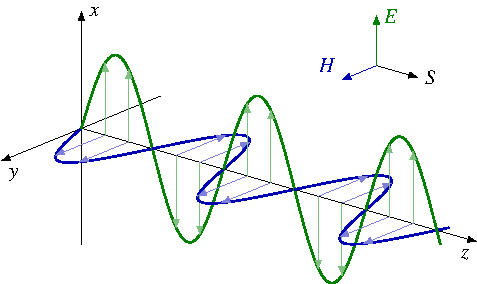
\includegraphics[width=100mm]{papers/opt/images/electromagnetic_wave_1.pdf}
    \caption{Die elektromagnetische Welle breitet sich in $z$-Richtung aus. 
    Wenn dabei die elektrische Feldstärke $\vec{E}$ entlang der $x$-Richtung verläuft, muss die magnetische Feldstärke $\vec{H}$ 
    in einem homogenen Medium orthogonal dazu entlang der $y$-Richtung verlaufen.}
    \label{opt:fig:electromagnetic_wave_1}
\end{figure}

Der Poynting-Vektor wird als
\begin{equation}
\vec{S} = \vec{E} \times \vec{H}
\label{opt:equation:poynting}
\end{equation}
definiert.
Er ist eie vektorielle Grösse für die Energie pro Fläche.
Dabei beschreibt $\vec{E}$ die elektrische und $\vec{H}$ die magnetische Feldstärke.
Um auf die gesuchte Intensität $I$ zu gelangen, muss die zeitlich gemittelte Leistung des Poynting-Vektors berechnet werden.

Angenommen eine elektromagnetische Welle breitet sich in $z$-Richtung in einem homogenen Medium aus, was unter anderem bedeutet, dass $\vec{E}$ und $\vec{H}$ immer orthogonal zueinander stehen müssen.
Verläuft nun die elektrische Feldstärke $\vec{E}$, wie in Abbildung \ref{opt:fig:electromagnetic_wave_1} gezeigt, entlang der $x$-Richtung, muss die magnetische Feldstärke $\vec{H}$ entlang der $y$-Richtung verlaufen.
Diese beiden Quantitäten können wiederum in komplexwertiger Notation, ähnlich zur Gleichung \eqref{opt:equation:wave}, als
\begin{equation}
\vec{E}(z,t)
=
E_0 \cdot e^{j(\omega t-k z)} \cdot \vec{x}
\label{opt:equation:wave_electric_field}
\end{equation}
und
\begin{equation}
\vec{H}(z,t)
=
H_0 \cdot e^{j(\omega t-k z)} \cdot \vec{y}
\label{opt:equation:wave_magnetic_field}
\end{equation}
geschrieben werden.
Eingesetzt in Gleichung \eqref{opt:equation:poynting} kann der Ausdruck als
\begin{align*}
\vec{S}
&=
\left(E_0 \cdot e^{j(\omega t-k z)} \cdot \vec{x}\right) \times \left(H_0 \cdot e^{j(\omega t-k z)} \cdot \vec{y}\right)
\\
&=
E_0 H_0 \cdot e^{2j(\omega t-k z)} \cdot \vec{z}
\\
&=
E_0 H_0 \cdot \left(\cos{(2(\omega t-kz))}+j\sin{(2(\omega t-kz))}\right) \vec{z}
\end{align*}
vereinfacht werden.

Da das zweite Moment des Real- oder Imaginärteils des Poynting-Vektors gerade der gesuchten Intensität $I$ entspricht, kann diese als 
\begin{align*}
I
&=
E(\Re^2(S))
=
E(\Im^2(S))
\\
&=
\frac{1}{t_1- t_0} \int_{t_0}^{t_1} \Re^2(S) \,dt
\\
&=
\frac{1}{t_1 - t_0} \cdot E_0 H_0 \cdot \int_{t_0}^{t_1}\cos\left({2(\omega t-kz)}\right)^2 \,dt
\\
&=
\frac{1}{t_1 - t_0} \cdot E_0 H_0 \cdot \int_{t_0}^{t_1}\frac{\cos(4(\omega t-kz)) + 1}{2} \,dt
\end{align*}
geschrieben werden.
Wenn nur über die Zeit gemittelt werden soll, ist die Position $z$ nicht relevant und kann daher auf $z = 0$ gesetzt werden.
Beispielsweise kann exakt über eine Periode integriert werden, was in Integrationsgrenzen von $t_0=0$ und
\begin{align*}
4\omega t_1
&=
2\pi
\\
t_1
&=
\frac{\pi}{2\omega}
\end{align*}
resultiert.
Mit den eingesetzten Grenzen ergibt sich der Ausdruck
\begin{align}
I
&=
\frac{1}{\frac{\pi}{2\omega} - 0} \cdot E_0 H_0 \cdot \int_{0}^{\frac{\pi}{2\omega}}\frac{\cos(4(\omega t-k\cdot0)) + 1}{2} \,dt
\notag
\\
&=
\frac{\omega}{\pi} \cdot E_0 H_0 \cdot \int_{0}^{\frac{\pi}{2\omega}}\cos(4\omega t) + 1 \,dt
\notag
\\
&=
\frac{\omega}{\pi} \cdot E_0 H_0 \cdot \left[\frac{\sin(4\omega t)}{4\omega} + t \right]_{0}^{\frac{\pi}{2\omega}}
\notag
\\
&=
\frac{\omega}{\pi} \cdot E_0 H_0 \cdot \left(\frac{\sin(2\pi)}{8\omega} + \frac{\pi}{2\omega}\right)
\notag
\\
&=
\frac{\omega}{\pi} \cdot E_0 H_0 \cdot \frac{\pi}{2\omega}
\notag
\\
&=
\frac{1}{2} \cdot E_0 H_0
\label{opt:equation:intensity_simple}
.
\end{align}

Dieser Ausdruck hängt jedoch noch von der magnetischen Feldstärke $H_0$ ab.
Ziel des nächsten Abschnittes wird es sein, mit Hilfe der Wellenimpedanz das Resultat \eqref{opt:equation:intensity_simple} von $H_0$ unabhängig zu schreiben.

%%%%%%%%%%%%%%%%%%%%%%%%%%%%%%%%%%%%%%%%%%%%%%%%%%%%%%%%%%%%%%%%%%%%%%%%%%%%%%%%%%%%%%%%%%%%%%%%%%%%%%%%%%%%%%%%%%%%%%%%
\subsection{Wellenimpedanz}
\label{opt:subsection:wave_impedance}
Die dritte Maxwellsche Gleichung, das Induktionsgesetz, lässt sich in Integralform als
\begin{equation}
\oint_{C=\partial A} \vec{E} \cdot\, d\vec{l}
=
-\frac{\partial}{\partial t} \int_{A} \vec{B} \cdot\, d\vec{s}
\label{opt:equation:maxwell_3}
\end{equation}
schreiben.
$B$ beschreibt dabei die magnetische Flussdichte, welche mit Hilfe der Permeabilität $\mu$ als $B = \mu H$ ausgedrückt werden kann.
Durch Abbildung \ref{opt:fig:electromagnetic_wave_2} ist die Umlaufspannung $u$ am Rand der Fläche $A$ gegeben durch
\begin{equation}
u
=
\oint_{C=\partial A} \vec{E} \cdot\, d\vec{l}
=
E_x(z+\Delta z,t) \cdot \Delta x - E_x(z,t) \cdot \Delta x
.
\label{opt:equation:induced_voltage}
\end{equation}
Nur Anteile des elektrischen Feldes in $x$-Richtung sind in diesem Resultat enthalten, da in den restlichen Richtungen das Skalarprodukt $\vec{E} \cdot d\vec{l} = 0$ ergibt, unabhängig von der gewählten Kontur $C = \partial A$.
Zusätzlich muss der magnetische Fluss $\Phi$ durch dieselbe Fläche $A$ bestimmt werden.
Dieser ergibt sich zu
\begin{equation}
\Phi
=
\int_{A} \vec{B} \cdot\, d\vec{s}
=
B_y\left(z+\frac{\Delta z}{2},t\right) \cdot \Delta x \,\Delta z
.
\label{opt:equation:magnetic_flux}
\end{equation}

\begin{figure}
    \centering
    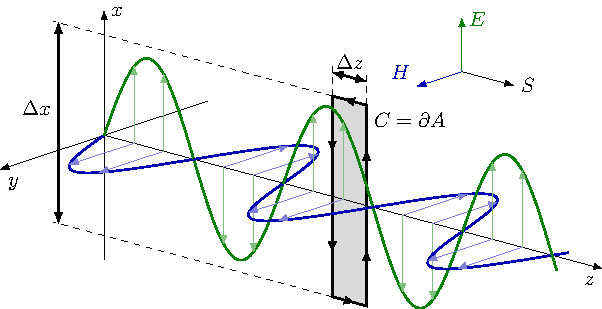
\includegraphics[width=100mm]{papers/opt/images/electromagnetic_wave_2.pdf}
    \caption{Grau eingefärbt ist die Fläche $A$, welche in der $xz$-Ebene liegt.
    Um sie herum verläuft in schwarz die Kontur $C = \partial A$.
    Zu beachten ist die Umlaufrichtung dieser Kontur, welche bestimmt, wann das Skalarprodukt $\vec{E} \cdot d\vec{l}$ ein positives oder negatives Vorzeichen aufweist.}
    \label{opt:fig:electromagnetic_wave_2}
\end{figure}

Wie zuvor bei der Umlaufspannung fallen hier nur Anteile der magnetischen Flussdichte in $y$-Richtung ins Gewicht.
Der Term $\frac{\Delta z}{2}$ wird hier dazu addiert, damit der Auswertungsort von $B_y$ exakt in der Mitte der Fläche $A$ liegt.
Die beiden erhaltenen Gleichungen \eqref{opt:equation:induced_voltage} und \eqref{opt:equation:magnetic_flux} können nun in Gleichung \eqref{opt:equation:maxwell_3} eingesetzt werden.
Woraus sich
\begin{align*}
u
&=
-\frac{\partial\Phi}{\partial t}
\\
E_x(z+\Delta z,t) \cdot \Delta x - E_x(z,t) \cdot \Delta x
&=
-\frac{\partial}{\partial t} B_y\left(z+\frac{\Delta z}{2},t\right) \cdot \Delta x \Delta z
\\
\frac{E_x(z+\Delta z,t) - E_x(z,t)}{\Delta z}
&=
-\frac{\partial}{\partial t} B_y\left(z+\frac{\Delta z}{2},t\right)
\end{align*}
ergibt.
Wird $\Delta z$ nun immer weiter verkleinert, kann auf beiden Seiten der Gleichung der Limes angewandt werden, woraus die Gleichung
\begin{align*}
\lim_{\Delta z \to 0} \frac{E_x(z+\Delta z,t) - E_x(z,t)}{\Delta z}
&=
-\lim_{\Delta z \to 0} \frac{\partial}{\partial t} B_y\left(z+\frac{\Delta z}{2},t\right)
\\
\frac{\partial E_x(z,t)}{\partial z}
&=
-\frac{\partial B_y(z,t)}{\partial t}
\end{align*}
resultiert.
Durch Einsetzen und Ableiten der Gleichungen \eqref{opt:equation:wave_electric_field} und \eqref{opt:equation:wave_magnetic_field} und unter Berücksichtigung von $B = \mu H$ und $\omega = kc$ ergibt sich schliesslich der Ausdruck
\begin{align}
-k \cdot E_0 \cdot e^{j(\omega t-k z)}
&=
-\mu \omega \cdot H_0 \cdot e^{j(\omega t-k z)}
\notag
\\
k \cdot E_0
&=
-\mu \omega \cdot H_0
\notag
\\
Z_0
=
\frac{E_0}{H_0}
&=
\frac{\mu \omega}{k}
=
\mu c
.
\label{opt:equation:impedance}
\end{align}

Dieses Verhältnis $Z_0$ von $E_0$ zu $H_0$ wird auch als Wellenimpedanz bezeichnet und spielt in der Elektrodynamik eine essentielle Rolle.
Ohne weiter darauf einzugehen, kann der Zusammenhang
\begin{equation}
c
=
\frac{1}{\sqrt{\varepsilon\mu}}
\label{opt:equation:speed_of_light}
\end{equation}
durch abermaliges Anwenden der Maxwellschen Gleichungen erhalten werden.
Wird nun Gleichung \eqref{opt:equation:speed_of_light} in \eqref{opt:equation:impedance} eingesetzt, kann durch Umformen der Ausdruck
\begin{equation}
\frac{E_0}{H_0}
=
\mu \frac{1}{\sqrt{\varepsilon\mu}}
=
\sqrt{\frac{\mu}{\varepsilon}}
=
\sqrt{\frac{\mu_r\mu_0}{\varepsilon_r\varepsilon_0}}
\label{opt:equation:impedance_simple}
\end{equation}
erhalten werden.
Bei der letzten Umformung wurden die Abhängigkeiten $\varepsilon = \varepsilon_r \varepsilon_0$ und $\mu = \mu_r \mu_0$ eingesetzt.
Die elektrische Feldkonstante $\varepsilon_0$ und die magnetische Feldkonstante $\mu_0$ sind beides Naturkonstanten und werden als
\begin{equation*}
\varepsilon_0
=
8.854 \cdot 10^{-12}
\end{equation*}
und
\begin{equation*}
\mu_0
=
4\pi \cdot 10^{-7}
\end{equation*}
definiert.
Die relative Permittivität $\varepsilon_r$ und die relative Permeabilität $\mu_r$ sind beides materialabhängige Faktoren und müssen je nach Medium, in welchem sich die Welle fortbewegt, nachgeschlagen und eingesetzt werden.

Wird Gleichung \eqref{opt:equation:impedance_simple} nach $H_0$ umgeformt und in \eqref{opt:equation:intensity_simple} eingesetzt, folgt für die Intensität schliesslich der Ausdruck
\begin{equation}
I
=
\frac{1}{2} \cdot E_0 H_0
=
\frac{1}{2} \cdot \sqrt{\frac{\varepsilon}{\mu}} \cdot E_0^2
=
\frac{1}{2} \cdot \sqrt{\frac{\varepsilon}{\mu}} \cdot |E|^2
=
\kappa \cdot |E|^2
,
\label{opt:equation:intensity}
\end{equation}
wobei der konstante Anteil als $\kappa$ zusammengefasst wurde.
Somit ist der einfachst mögliche Zusammenhang zwischen der elektrischen Feldstärke $E$ und der Intensität $I$ gefunden.
Die Intensität an einer bestimmten Stelle im Raum ist also lediglich abhängig von der an diesem Ort herrschenden elektrischen Feldstärke $E$ und der Medium spezifischen Konstante $\kappa$.

%%%%%%%%%%%%%%%%%%%%%%%%%%%%%%%%%%%%%%%%%%%%%%%%%%%%%%%%%%%%%%%%%%%%%%%%%%%%%%%%%%%%%%%%%%%%%%%%%%%%%%%%%%%%%%%%%%%%%%%%
\subsection{Rechenbeispiel zur Beugung am Einzelspalt}
\label{opt:sec:exampleSingleSlit}
Als einfachstes Beispiel wird die Beugung an einem einzelnen Spalt der Breite $b$ durchexerziert.
In diesem Fall beträgt die Blendenfunktion
\begin{equation*}
f(y)
=
\begin{cases}
1 & \text{für } -\frac{b}{2} \leq x \leq \frac{b}{2} \\
0 & \text{sonst}
\end{cases}
.
\end{equation*}
Als Ausgangslage wird die Gleichung \eqref{opt:equation:intensity} aus dem vorhergehenden Abschnitt verwendet.
Wenn dabei die elektrische Feldstärke $\vec{E}$ durch die Fraunhofer-Approximation aus \eqref{opt:equation:integral_fraunhofer} ausgedrückt wird, kann die Gleichung als
\begin{align*}
I(y_p)
&=
\kappa \cdot |E|^2
=
\kappa \cdot \frac{\vartheta^2\zeta_0^2}{l^2}\cdot \left|\int_{-\infty}^{\infty}f(y)\cdot e^{-j\frac{ky_p}{l}y} \,dy\right|^2
\intertext{geschrieben werden. Durch Einsetzen der Grenzen vereinfacht sich diese zu}
&=
\kappa \cdot \frac{\vartheta^2\zeta_0^2}{l^2}\cdot \Biggl|\int_{-\frac{b}{2}}^{\frac{b}{2}}e^{-j\frac{ky_p}{l}y} \,dy\Biggr|^2.
\intertext{Anschliessend kann die Stammfunktion an den Grenzen ausgewertet werden.}
&=
\kappa \cdot \frac{\vartheta^2\zeta_0^2}{l^2}\cdot \left|-\frac{l}{jky_p} \cdot \left[e^{-j\frac{ky_p}{l}y} \right]_{y=-\frac{b}{2}}^{y=\frac{b}{2}}\right|^2
\\
&=
\kappa \cdot \frac{\vartheta^2\zeta_0^2}{l^2}\cdot \left|-\frac{l}{jky_p} \cdot \left(e^{-j\frac{bky_p}{2l}} - e^{-j\frac{-bky_p}{2l}}\right)\right|^2
\\
&=
\kappa \cdot \frac{\vartheta^2\zeta_0^2}{l^2}\cdot \left|-\frac{l}{jky_p} \cdot \left(e^{-j\frac{bky_p}{2l}} - e^{j\frac{bky_p}{2l}}\right)\right|^2
\\
&=
\kappa \cdot \frac{\vartheta^2\zeta_0^2}{l^2}\cdot \left|\frac{2bl}{bky_p} \cdot \frac{1}{2j} \cdot \left(e^{j\frac{bky_p}{2l}} - e^{-j\frac{bky_p}{2l}}\right)\right|^2
\end{align*}
Der daraus entstandene Ausdruck kann mit Hilfe der Eulerschen Identität des Sinus
\begin{equation*}
\sin(x) = \frac{e^{jx} - e^{-jx}}{2j}
\end{equation*}
und der Definition der $\sinc$ Funktion
\begin{equation*}
\sinc(x) = \frac{\sin(x)}{x}
\end{equation*}
weiter zu
\begin{align*}
I(y_p)
&=
\kappa \cdot \frac{\vartheta^2\zeta_0^2}{l^2}\cdot \left(\frac{2bl}{bky_p} \cdot \sin\left(\frac{bky_p}{2l}\right)\right)^2
\\
&=
\kappa \cdot \frac{\vartheta^2\zeta_0^2}{l^2}\cdot b^2 \cdot \sinc^2\left(\frac{bky_p}{2l}\right)
.
\end{align*}
vereinfacht werden.

Die Fraunhofer-Approximation aus \eqref{opt:equation:integral_fraunhofer}, ausgewertet für einen Einzelspalt, ergibt schlussendlich eine quadrierte sinc-Funktion.
Das hier erhaltene Schlussresultat wird in Abschnitt \ref{opt:section:versuch} praktisch nachgewiesen.
